\documentclass[11pt,a4paper]{article}

% ───────────────────────── Packages ─────────────────────────
\usepackage[utf8]{inputenc}
\usepackage[T1]{fontenc}
\usepackage{lmodern}
\usepackage[margin=2cm]{geometry}
\usepackage{graphicx}
\usepackage{xcolor}
\usepackage{tikz}
\usetikzlibrary{
  arrows.meta, positioning, shapes.geometric, shapes.misc,
  fit, calc, backgrounds, decorations.pathreplacing,
  decorations.markings, patterns
}
\usepackage{pgfplots}
\pgfplotsset{compat=1.18}
\usepackage[ruled,vlined,linesnumbered]{algorithm2e}
\usepackage{listings}
\usepackage{booktabs}
\usepackage{amsmath,amssymb}
\usepackage{enumitem}
\usepackage{hyperref}
\usepackage{float}
\usepackage{subcaption}
\usepackage{fancyhdr}
\usepackage{tcolorbox}
\tcbuselibrary{skins,breakable,listings}
\usepackage{multicol}

% ───────────────────────── Colors ─────────────────────────
\definecolor{popA}{RGB}{31,119,180}
\definecolor{popB}{RGB}{214,39,40}
\definecolor{redis}{RGB}{220,50,47}
\definecolor{codebg}{RGB}{248,248,248}
\definecolor{armA}{RGB}{44,160,44}
\definecolor{armC}{RGB}{148,103,189}
\definecolor{highlight}{RGB}{255,127,14}
\definecolor{stageblue}{RGB}{66,133,244}
\definecolor{darkgreen}{RGB}{0,128,0}

% ───────────────────────── Listings ─────────────────────────
\lstdefinestyle{pythonstyle}{
  language=Python,
  backgroundcolor=\color{codebg},
  basicstyle=\ttfamily\scriptsize,
  keywordstyle=\color{blue}\bfseries,
  stringstyle=\color{darkgreen},
  commentstyle=\color{gray}\itshape,
  numberstyle=\tiny\color{gray},
  numbers=left, numbersep=5pt,
  breaklines=true, breakatwhitespace=true,
  frame=single, framesep=3pt,
  rulecolor=\color{lightgray},
  showstringspaces=false, tabsize=4,
  captionpos=b, xleftmargin=1.5em, framexleftmargin=1.5em,
  aboveskip=0.8em, belowskip=0.5em,
}
\lstset{style=pythonstyle}

% ───────────────────────── tcolorbox ─────────────────────────
\newtcolorbox{eli5box}[1][]{
  colback=yellow!5!white, colframe=yellow!75!black,
  fonttitle=\bfseries, title={Intuition}, #1
}
\newtcolorbox{designbox}[1][]{
  colback=blue!3!white, colframe=popA!80!black,
  fonttitle=\bfseries, #1
}

% ───────────────────────── Headers ─────────────────────────
\pagestyle{fancy}
\fancyhf{}
\fancyhead[L]{\small\textsc{GigaEvo Adversarial Architecture}}
\fancyhead[R]{\small\thepage}
\renewcommand{\headrulewidth}{0.4pt}

% ───────────────────────── Math shortcuts ─────────────────────────
\newcommand{\Qstar}{Q^{*}}      % conjectured optimum (replaces Q_MAX)
\newcommand{\minarea}{\operatorname{min\_area}}

% ═══════════════════════════════════════════════════════════
\title{%
  \vspace{-1cm}
  {\LARGE\bfseries Adversarial Co-Evolution Architecture}\\[0.3cm]
  {\Large GigaEvo Framework --- Technical Report}\\[0.3cm]
  {\normalsize Heilbronn $N\!=\!11$ Triangle Experiment}
}
\author{%
  GigaEvo Research Team\\
  {\small Experiment: \texttt{heilbron/asymmetric-iterations} (PR~\#204)}
}
\date{April 12, 2026}

\begin{document}
\maketitle
\thispagestyle{fancy}

% ═══════════════════════════════════════════════════════════
\section{What This System Does (Plain English)}
% ═══════════════════════════════════════════════════════════

\begin{eli5box}
\textbf{Imagine two teams playing a game:}
\begin{itemize}[nosep]
  \item \textbf{Team~G (Constructors, blue):} Place 11 points inside a triangle so that no three points form a tiny triangle. Think of it as ``spread them out as evenly as possible.''
  \item \textbf{Team~D (Improvers, red):} Take G's arrangement and rearrange points to make the smallest triangle \emph{bigger}. If D can improve G's layout, G was not optimal.
\end{itemize}

Both teams are \emph{populations of evolving programs}. An LLM (large language model) writes Python code that gets tested, scored, and selectively bred --- just like biological evolution, but with code instead of DNA.

The key insight: \textbf{G and D push each other to improve.} G evolves configurations that are harder and harder to improve. D evolves strategies that crack increasingly tough configurations. This is analogous to how GANs work in deep learning, but here the ``networks'' are explicit Python programs evolved by an LLM.
\end{eli5box}

% ═══════════════════════════════════════════════════════════
\section{Background: The Heilbronn Triangle Problem}
% ═══════════════════════════════════════════════════════════

The Heilbronn triangle problem asks: \emph{given $n$ points in a convex region, what is the maximum possible value of the smallest triangle area formed by any three of them?}

For $n=11$ in a unit-area equilateral triangle ($A{=}(0,0),\; B{=}(1.52,0),\; C{=}(0.76,1.32)$), the conjectured optimum is $\Qstar \approx 0.0365$.

\begin{figure}[H]
\centering
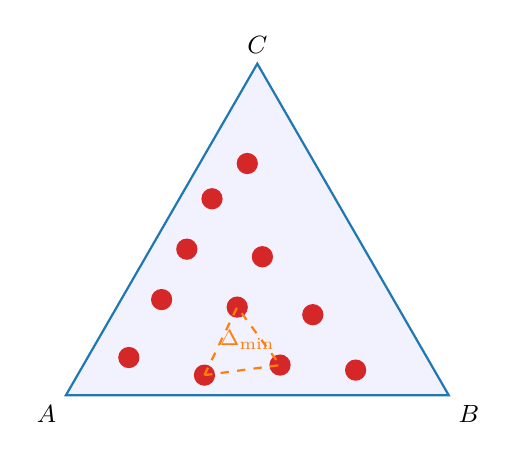
\begin{tikzpicture}[scale=3.2]
  \fill[blue!5] (0,0) -- (1.5197,0) -- (0.7598,1.3161) -- cycle;
  \draw[thick,popA] (0,0) -- (1.5197,0) -- (0.7598,1.3161) -- cycle;
  \foreach \x/\y in {0.25/0.15, 0.55/0.08, 0.85/0.12, 1.15/0.10,
                      0.38/0.38, 0.68/0.35, 0.98/0.32,
                      0.48/0.58, 0.78/0.55, 0.58/0.78, 0.72/0.92} {
    \fill[popB] (\x,\y) circle (1.2pt);
  }
  \draw[highlight,thick,dashed] (0.55,0.08) -- (0.68,0.35) -- (0.85,0.12) -- cycle;
  \node[highlight,font=\footnotesize] at (0.72,0.22) {$\Delta_{\min}$};
  \node[below left,font=\small] at (0,0) {$A$};
  \node[below right,font=\small] at (1.5197,0) {$B$};
  \node[above,font=\small] at (0.7598,1.3161) {$C$};
\end{tikzpicture}
\caption{Heilbronn $N\!=\!11$: place 11 points to maximize $\Delta_{\min}$.}
\label{fig:heilbronn}
\end{figure}

% ═══════════════════════════════════════════════════════════
\section{System Architecture Overview}
% ═══════════════════════════════════════════════════════════

\begin{figure}[H]
\centering
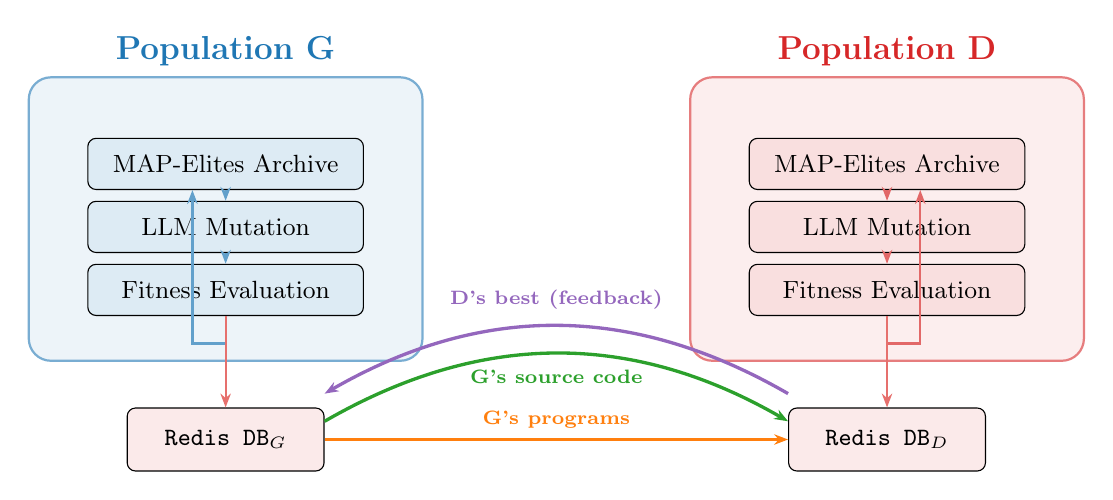
\begin{tikzpicture}[
    pop/.style={draw,rounded corners=8pt,minimum width=5cm,minimum height=3.6cm,thick},
    stage/.style={draw,rounded corners=3pt,fill=white,minimum width=3.5cm,
      minimum height=0.65cm,font=\small},
    redis/.style={draw,fill=redis!10,rounded corners=3pt,minimum width=2.5cm,
      font=\small\ttfamily},
    arrow/.style={-{Stealth[length=5pt]},thick},
    >=Stealth
  ]

  % Population G
  \node[pop,fill=popA!8,draw=popA!60] (popG) at (-4.2,0) {};
  \node[above,font=\bfseries\large,popA] at (popG.north) {Population G};
  \node[font=\small,popA] at ([yshift=-3pt]popG.north) {\strut};
  \node[stage,fill=popA!15] (gevo) at (-4.2,0.7) {MAP-Elites Archive};
  \node[stage,fill=popA!15] (gmut) at (-4.2,-0.1) {LLM Mutation};
  \node[stage,fill=popA!15] (geval) at (-4.2,-0.9) {Fitness Evaluation};

  % Population D
  \node[pop,fill=popB!8,draw=popB!60] (popD) at (4.2,0) {};
  \node[above,font=\bfseries\large,popB] at (popD.north) {Population D};
  \node[stage,fill=popB!15] (devo) at (4.2,0.7) {MAP-Elites Archive};
  \node[stage,fill=popB!15] (dmut) at (4.2,-0.1) {LLM Mutation};
  \node[stage,fill=popB!15] (deval) at (4.2,-0.9) {Fitness Evaluation};

  % Redis
  \node[redis,minimum height=0.8cm] (rg) at (-4.2,-2.8) {Redis DB$_G$};
  \node[redis,minimum height=0.8cm] (rd) at (4.2,-2.8) {Redis DB$_D$};

  % Internal arrows
  \draw[arrow,popA!70] (gevo) -- (gmut);
  \draw[arrow,popA!70] (gmut) -- (geval);
  \draw[arrow,popA!70] (geval.south) -- ++(0,-0.35) -| ([xshift=-12pt]gevo.south);

  \draw[arrow,popB!70] (devo) -- (dmut);
  \draw[arrow,popB!70] (dmut) -- (deval);
  \draw[arrow,popB!70] (deval.south) -- ++(0,-0.35) -| ([xshift=12pt]devo.south);

  % Redis connections
  \draw[arrow,redis!70] (geval.south) -- (rg);
  \draw[arrow,redis!70] (deval.south) -- (rd);

  % Cross-population: G's programs -> D's evaluator
  \draw[arrow,highlight,very thick]
    (rg.east) -- node[above,font=\scriptsize\bfseries,highlight] {G's programs} (rd.west);

  % Cross-population: D's best -> G's mutation prompt (Arm C)
  \draw[arrow,armC,very thick]
    ([yshift=5pt]rd.north west) to[out=150,in=30]
    node[above,font=\scriptsize\bfseries,armC,yshift=2pt] {D's best (feedback)}
    ([yshift=5pt]rg.north east);

  % Cross-population: G's source -> D's mutation prompt
  \draw[arrow,armA,very thick]
    ([yshift=-5pt]rg.north east) to[out=30,in=150]
    node[below,font=\scriptsize\bfseries,armA,yshift=-2pt] {G's source code}
    ([yshift=-5pt]rd.north west);

\end{tikzpicture}
\caption{Two-population adversarial co-evolution. Each population runs an independent MAP-Elites loop. Communication flows through Redis: G's programs are sampled as test cases for D (orange); D's best strategies provide feedback to G (purple, Arm~C only); G's source code is shown to D (green).}
\label{fig:architecture}
\end{figure}

\subsection{How MAP-Elites Works}

\begin{eli5box}
Think of MAP-Elites as a ``hall of fame'' of diverse programs.  Instead of keeping just the single best, it keeps the best program \emph{in each niche} (cell of a quality-diversity grid).  This prevents collapse to a single strategy and encourages diverse approaches.
\end{eli5box}

\begin{algorithm}[H]
\SetAlgoLined\DontPrintSemicolon
\caption{MAP-Elites Evolution Loop (per population)}
\label{alg:mapelites}
\KwIn{Archive $\mathcal{A}$, LLM mutation operator $\mu$, max generations $G$}
\For{$g = 1$ \KwTo $G$}{
  \texttt{pre\_step\_hook()} \tcp*{Sync with opponent}
  $\mathcal{E} \leftarrow$ \texttt{select\_elites}$(\mathcal{A})$ \tcp*{Fitness-proportional}
  \For{each $p \in \mathcal{E}$}{
    $p' \leftarrow \mu(p)$ \tcp*{LLM rewrites program}
    Run DAG pipeline: validate $\to$ execute $\to$ evaluate\;
    \lIf{$p'$ valid \textbf{and} better than $\mathcal{A}[\text{cell}(p')]$}{
      $\mathcal{A}[\text{cell}(p')] \leftarrow p'$}
  }
  Refresh archive (re-evaluate against current opponents)\;
}
\end{algorithm}

% ═══════════════════════════════════════════════════════════
\section{The DAG Pipeline}
% ═══════════════════════════════════════════════════════════

Each candidate program is evaluated through a DAG of processing stages. The adversarial pipeline extends the standard pipeline with opponent-interaction stages.

\begin{figure}[H]
\centering
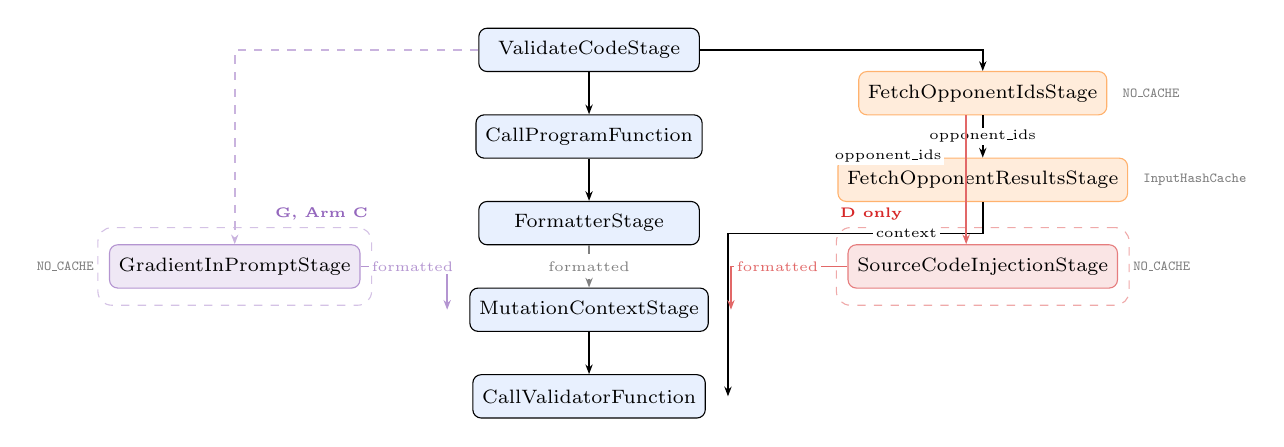
\begin{tikzpicture}[
    stage/.style={draw,rounded corners=3pt,fill=stageblue!12,
      minimum width=2.8cm,minimum height=0.55cm,font=\scriptsize,align=center},
    advstage/.style={draw,rounded corners=3pt,fill=highlight!15,draw=highlight!60,
      minimum width=2.8cm,minimum height=0.55cm,font=\scriptsize,align=center},
    injstage/.style={draw,rounded corners=3pt,fill=popB!12,draw=popB!60,
      minimum width=2.8cm,minimum height=0.55cm,font=\scriptsize,align=center},
    gradstage/.style={draw,rounded corners=3pt,fill=armC!15,draw=armC!70,
      minimum width=2.8cm,minimum height=0.55cm,font=\scriptsize,align=center},
    arrow/.style={-{Stealth[length=3.5pt]},semithick},
    darrow/.style={-{Stealth[length=3.5pt]},semithick,dashed,gray},
    lbl/.style={font=\tiny,fill=white,inner sep=1pt},
    cache/.style={font=\tiny\ttfamily,gray},
    >=Stealth
  ]

  % Standard stages (center column)
  \node[stage] (validate) at (0,0) {ValidateCodeStage};
  \node[stage] (callprog) at (0,-1.1) {CallProgramFunction};
  \node[stage] (format) at (0,-2.2) {FormatterStage};
  \node[stage] (mutctx) at (0,-3.3) {MutationContextStage};
  \node[stage] (callval) at (0,-4.4) {CallValidatorFunction};

  % Adversarial stages (right column, wider gap)
  \node[advstage] (fetchids) at (5,-0.55) {FetchOpponentIdsStage};
  \node[cache,right=2pt of fetchids] {NO\_CACHE};
  \node[advstage] (fetchres) at (5,-1.65) {FetchOpponentResultsStage};
  \node[cache,right=2pt of fetchres] {InputHashCache};

  % D-only: SourceCodeInjection (below, right)
  \node[injstage] (srcinj) at (5,-2.75) {SourceCodeInjectionStage};
  \node[cache,right=2pt of srcinj] {NO\_CACHE};

  % G-only (Arm C): GradientInPrompt (left column)
  \node[gradstage] (gradient) at (-4.5,-2.75) {GradientInPromptStage};
  \node[cache,left=2pt of gradient] {NO\_CACHE};

  % Standard flow
  \draw[arrow] (validate) -- (callprog);
  \draw[arrow] (callprog) -- (format);
  \draw[darrow] (format) -- node[lbl] {formatted} (mutctx);
  \draw[arrow] (mutctx) -- (callval);

  % Adversarial flow
  \draw[arrow] (validate.east) -| (fetchids.north);
  \draw[arrow] (fetchids) -- node[lbl] {opponent\_ids} (fetchres);
  \draw[arrow] (fetchres.south) -- ++(0,-0.4) -| ([xshift=8pt]callval.east)
    node[lbl,pos=0.15] {context};

  % Fork: IDs -> SourceCodeInjection
  \draw[arrow,popB!70] ([xshift=-6pt]fetchids.south) -- ++(0,-0.25)
    -| ([xshift=-6pt]srcinj.north);
  \node[lbl] at (3.8,-1.35) {opponent\_ids};

  % SourceCodeInjection -> MutationContext
  \draw[arrow,popB!70] (srcinj.west) -| node[lbl,pos=0.3] {formatted}
    ([xshift=8pt]mutctx.east);

  % Gradient -> MutationContext
  \draw[arrow,armC!70] (gradient.east) -| node[lbl,pos=0.3] {formatted}
    ([xshift=-8pt]mutctx.west);

  % Gradient trigger
  \draw[arrow,armC!50,dashed] (validate.west) -| (gradient.north);

  % Dashed region labels
  \begin{scope}[on background layer]
    \node[draw=popB!40,dashed,rounded corners=5pt,fit=(srcinj),
      inner xsep=4pt,inner ysep=6pt] (dbox) {};
    \node[popB,font=\tiny\bfseries,above right=-1pt and -2pt of dbox.north west] {D only};
    \node[draw=armC!40,dashed,rounded corners=5pt,fit=(gradient),
      inner xsep=4pt,inner ysep=6pt] (gbox) {};
    \node[armC,font=\tiny\bfseries,above left=-1pt and -2pt of gbox.north east] {G, Arm~C};
  \end{scope}
\end{tikzpicture}
\caption{Asymmetric adversarial DAG.  Orange = shared adversarial stages.  Red = D-only (source injection).  Purple = G-only, Arm~C (gradient).  \textbf{Fork}: \texttt{FetchOpponentIdsStage} feeds \emph{both} evaluation and source injection paths.}
\label{fig:dag}
\end{figure}

\begin{eli5box}
\textbf{The DAG is like an assembly line.} Each program passes through stations: syntax check $\to$ execution $\to$ formatting $\to$ opponent testing $\to$ final scoring. D gets an extra station that reads G's source code (white-box access). In Arm~C, G gets a station that reads D's best code (bidirectional white-box).
\end{eli5box}

\subsection{Caching Strategy}

\begin{table}[H]
\centering\small
\begin{tabular}{@{}lll@{}}
\toprule
\textbf{Stage} & \textbf{Cache} & \textbf{Why} \\
\midrule
FetchOpponentIdsStage & \texttt{NO\_CACHE} & Must re-sample fresh opponents \\
FetchOpponentResultsStage & \texttt{InputHashCache} & Re-run only when IDs change \\
SourceCodeInjectionStage & \texttt{NO\_CACHE} & Opponent code evolves \\
GradientInPromptStage & \texttt{NO\_CACHE} & D's best changes continuously \\
\bottomrule
\end{tabular}
\caption{Cache policies. \texttt{NO\_CACHE} = always re-execute; \texttt{InputHashCache} = re-execute when input hash changes.}
\end{table}

% ═══════════════════════════════════════════════════════════
\section{Cross-Population Communication}
% ═══════════════════════════════════════════════════════════

The two populations communicate exclusively through Redis.

\begin{figure}[H]
\centering
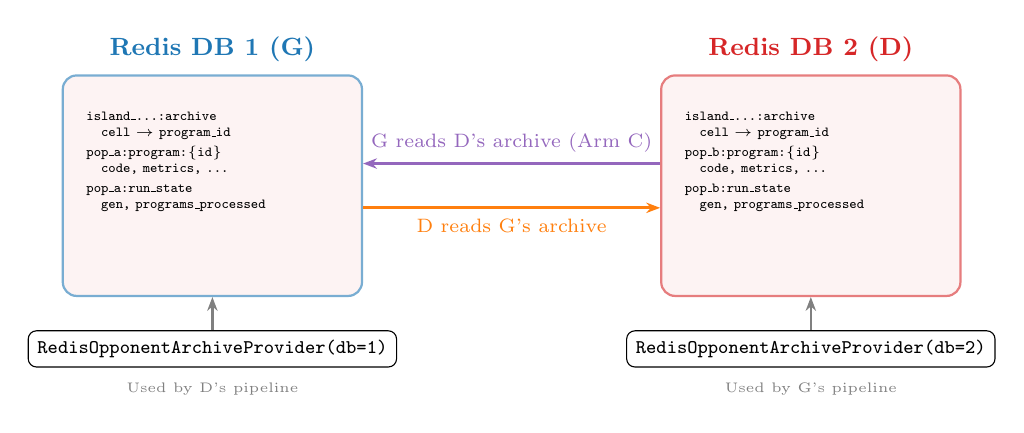
\begin{tikzpicture}[
    db/.style={draw,fill=redis!6,rounded corners=5pt,
      minimum width=3.8cm,minimum height=2.8cm,thick},
    kv/.style={font=\ttfamily\tiny,text width=3.2cm},
    prov/.style={draw,rounded corners=3pt,fill=white,font=\scriptsize\ttfamily},
    arrow/.style={-{Stealth[length=5pt]},thick},
    >=Stealth
  ]

  % DB G
  \node[db,draw=popA!60] (dbg) at (-3.8,0) {};
  \node[above=1pt,font=\bfseries\small,popA] at (dbg.north) {Redis DB 1 (G)};
  \node[kv,anchor=north] at ([yshift=-10pt]dbg.north) {%
    island\_...:archive\\
    \quad cell $\to$ program\_id\\[1pt]
    pop\_a:program:\{id\}\\
    \quad code, metrics, \ldots\\[1pt]
    pop\_a:run\_state\\
    \quad gen, programs\_processed
  };

  % DB D
  \node[db,draw=popB!60] (dbd) at (3.8,0) {};
  \node[above=1pt,font=\bfseries\small,popB] at (dbd.north) {Redis DB 2 (D)};
  \node[kv,anchor=north] at ([yshift=-10pt]dbd.north) {%
    island\_...:archive\\
    \quad cell $\to$ program\_id\\[1pt]
    pop\_b:program:\{id\}\\
    \quad code, metrics, \ldots\\[1pt]
    pop\_b:run\_state\\
    \quad gen, programs\_processed
  };

  % Cross-read arrows (stacked vertically to avoid overlap)
  \draw[arrow,highlight,very thick]
    ([yshift=-8pt]dbg.east) -- node[below,font=\scriptsize,highlight]
      {D reads G's archive} ([yshift=-8pt]dbd.west);
  \draw[arrow,armC,very thick]
    ([yshift=8pt]dbd.west) -- node[above,font=\scriptsize,armC]
      {G reads D's archive (Arm~C)} ([yshift=8pt]dbg.east);

  % Providers
  \node[prov,below=12pt of dbg] (provG) {RedisOpponentArchiveProvider(db=1)};
  \node[prov,below=12pt of dbd] (provD) {RedisOpponentArchiveProvider(db=2)};
  \draw[arrow,gray] (provG) -- (dbg);
  \draw[arrow,gray] (provD) -- (dbd);
  \node[font=\tiny,gray,below=2pt of provG] {Used by D's pipeline};
  \node[font=\tiny,gray,below=2pt of provD] {Used by G's pipeline};
\end{tikzpicture}
\caption{Redis-mediated cross-population communication.  Cache TTL = 30\,s.}
\label{fig:redis}
\end{figure}

\subsection{Opponent Sampling}

Opponents are sampled using \textbf{softmax fitness-proportional selection}:

\begin{lstlisting}[caption={Softmax sampling (\texttt{opponent\_provider.py:23--41})}]
def _softmax_weights(fitnesses: list[float]) -> list[float]:
    arr = np.asarray(fitnesses, dtype=np.float64)
    fitness_range = float(np.ptp(arr))
    if fitness_range < 1e-10:
        return [1.0 / len(arr)] * len(arr)  # uniform
    arr = (arr - arr.min()) / fitness_range  # normalize
    std = float(np.std(arr, ddof=1)) if len(arr) > 1 else 0.0
    temp = max(std, 0.01)                    # auto-temperature
    return softmax(arr / temp).tolist()
\end{lstlisting}

% ═══════════════════════════════════════════════════════════
\section{The Two Treatment Arms}
% ═══════════════════════════════════════════════════════════

The experiment compares two mechanisms by which D's discoveries flow back to G.

\begin{figure}[H]
\centering
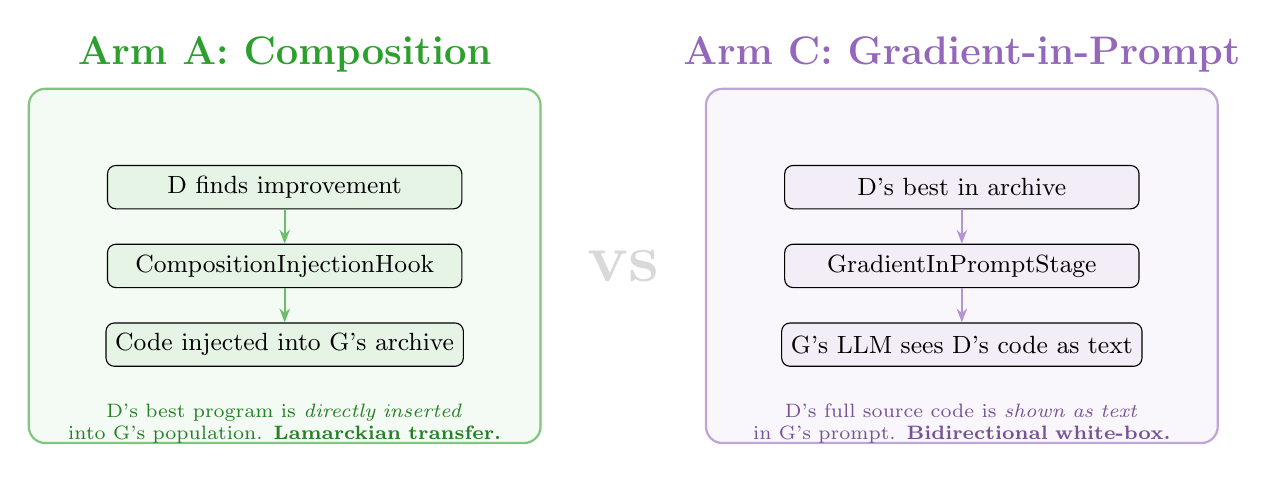
\begin{tikzpicture}[
    box/.style={draw,rounded corners=6pt,minimum width=6.5cm,minimum height=4.5cm,thick},
    stage/.style={draw,rounded corners=3pt,fill=white,
      minimum width=4.5cm,minimum height=0.55cm,font=\small},
    arrow/.style={-{Stealth[length=5pt]},thick},
    >=Stealth
  ]

  % Arm A
  \node[box,fill=armA!5,draw=armA!60] (armAbox) at (-4.3,0) {};
  \node[above=2pt,font=\Large\bfseries,armA] at (armAbox.north) {Arm A: Composition};

  \node[stage,fill=armA!12] (a1) at (-4.3,1) {D finds improvement};
  \node[stage,fill=armA!12] (a2) at (-4.3,0) {CompositionInjectionHook};
  \node[stage,fill=armA!12] (a3) at (-4.3,-1) {Code injected into G's archive};
  \draw[arrow,armA!70] (a1) -- (a2);
  \draw[arrow,armA!70] (a2) -- (a3);

  \node[font=\scriptsize,text width=5.5cm,align=center,armA!80!black] at (-4.3,-2) {
    D's best program is \emph{directly inserted}\\
    into G's population. \textbf{Lamarckian transfer.}
  };

  % Arm C
  \node[box,fill=armC!5,draw=armC!60] (armCbox) at (4.3,0) {};
  \node[above=2pt,font=\Large\bfseries,armC] at (armCbox.north) {Arm C: Gradient-in-Prompt};

  \node[stage,fill=armC!12] (c1) at (4.3,1) {D's best in archive};
  \node[stage,fill=armC!12] (c2) at (4.3,0) {GradientInPromptStage};
  \node[stage,fill=armC!12] (c3) at (4.3,-1) {G's LLM sees D's code as text};
  \draw[arrow,armC!70] (c1) -- (c2);
  \draw[arrow,armC!70] (c2) -- (c3);

  \node[font=\scriptsize,text width=5.5cm,align=center,armC!80!black] at (4.3,-2) {
    D's full source code is \emph{shown as text}\\
    in G's prompt. \textbf{Bidirectional white-box.}
  };

  % VS
  \node[font=\Huge\bfseries,gray!30] at (0,0) {vs};
\end{tikzpicture}
\caption{Arm~A directly transplants D's code into G's archive (Lamarckian --- G does not see D's source).  Arm~C shows D's full source code as text in G's LLM prompt (Baldwinian --- G has white-box access to D). The hypothesis: the transfer mechanism significantly affects arms-race dynamics.}
\label{fig:arms}
\end{figure}

\subsection{Arm A: Composition Injection}

\begin{lstlisting}[caption={CompositionInjectionHook (\texttt{composition\_injection.py:36--61})}]
async def inject(self) -> str | None:
    """Read D's best and submit to G's population."""
    top = await self._d_provider.get_top_k(1, higher_is_better=True)
    if not top:
        return None
    d_best = top[0]
    program = Program(
        code=d_best.code,
        metadata={"mutation_type": "d_improvement",
                  "d_source_id": d_best.program_id,
                  "d_fitness": d_best.fitness},
    )
    await self._g_storage.add(program)
    return program.id
\end{lstlisting}

\subsection{Arm C: Gradient-in-Prompt}

\begin{lstlisting}[caption={GradientInPromptStage prompt (\texttt{gradient\_prompt.py:24--42})}]
_GRADIENT_HEADER = """\
## Improvement Strategy from Opponent

The following Improver program has been the most
effective at finding improvements to Constructor
configurations like yours. Study its approach to
understand what weaknesses it exploits, then evolve
your strategy to resist these attacks.

**Improver fitness**: {fitness:.5f}\
"""
# ... followed by the full Python source of D's best
\end{lstlisting}

% ═══════════════════════════════════════════════════════════
\section{White-Box Access: Both Populations See Source Code}
% ═══════════════════════════════════════════════════════════

Both populations get white-box access to their opponent's source code, though through different mechanisms:

\begin{itemize}[nosep]
  \item \textbf{D always sees G's code} via \texttt{SourceCodeInjectionStage} (both arms).
  \item \textbf{G sees D's code in Arm~C} via \texttt{GradientInPromptStage} --- D's best Improver source code is shown in G's mutation prompt as a ``textual gradient.''
\end{itemize}

In Arm~A (composition), G does \emph{not} see D's source --- instead D's code is directly injected into G's archive as a candidate program.

\begin{eli5box}
Both populations can read their opponent's Python source code --- not just outputs. D studies G's point-placement algorithm to find weaknesses. In Arm~C, G studies D's improvement algorithm to evolve resistance.  This is like two chess players who can see each other's strategy notebooks.
\end{eli5box}

\subsection{D's Source Injection (Fork Topology)}

The fork topology is key: \texttt{FetchOpponentIdsStage} outputs one ID list that feeds \emph{both}:
\begin{enumerate}[nosep]
  \item \textbf{FetchOpponentResultsStage} --- runs G's code $\to$ point configs for evaluation
  \item \textbf{SourceCodeInjectionStage} --- fetches G's source code for the prompt
\end{enumerate}
Same opponents for evaluation and source reading --- no conceptual leakage.

\begin{lstlisting}[caption={Fork wiring (\texttt{asymmetric\_pipeline.py:109--133})}]
def _add_source_injection(self, opponent_provider,
                          source_prompt_k, stage_timeout):
    self.remove_data_flow_edge(
        "FormatterStage", "MutationContextStage")
    self.add_stage("SourceCodeInjectionStage",
        lambda: SourceCodeInjectionStage(
            opponent_provider=opponent_provider,
            source_prompt_k=source_prompt_k,
            timeout=stage_timeout))
    # Fork: same IDs -> both eval and injection
    self.add_data_flow_edge("FetchOpponentIdsStage",
        "SourceCodeInjectionStage", "opponent_ids")
    self.add_data_flow_edge("SourceCodeInjectionStage",
        "MutationContextStage", "formatted")
\end{lstlisting}

% ═══════════════════════════════════════════════════════════
\section{Generational Synchronization}
% ═══════════════════════════════════════════════════════════

\begin{algorithm}[H]
\SetAlgoLined\DontPrintSemicolon
\caption{ProgressBasedSyncHook (pre-step hook)}
\label{alg:sync}
\KwIn{Opponent Redis sources, $\delta_{\min}$, $K$ (sync every $K$ epochs)}
$\text{count} \leftarrow \text{count} + 1$\;
\lIf{$\text{count} < K$}{\Return \tcp*{asymmetric ratio}}
$\text{count} \leftarrow 0$\;
\lIf{first call}{record baseline, \Return}
$\text{target} \leftarrow \text{baseline} + \delta_{\min}$\;
\While{$\min\_progress(\text{sources}) < \text{target}$}{
  \lIf{elapsed $>$ timeout}{\textbf{warn}, proceed}
  \texttt{sleep}(poll\_interval)\;
}
$\text{baseline} \leftarrow \min\_progress(\text{sources})$\;
\end{algorithm}

\begin{eli5box}
\textbf{Buddy system.}  Before each generation, a population checks: ``Has my opponent made progress?''  If not, it waits.  The \texttt{sync\_every\_n\_epochs} parameter supports asymmetric ratios (e.g., D updates 3$\times$ per G update).
\end{eli5box}

% ═══════════════════════════════════════════════════════════
\section{Fitness Functions}
% ═══════════════════════════════════════════════════════════

Let $\Qstar \approx 0.0365$ denote the conjectured global optimum for $N\!=\!11$.

\subsection{Constructor (G)}

\begin{equation}
  \text{fitness}_G = \frac{1}{2}\underbrace{\min\!\left(\frac{\minarea(\text{config})}{\Qstar},\; 1\right)}_{\text{quality}\;(\text{how close to }\Qstar)} + \;\frac{1}{2}\underbrace{\frac{|\{k : \Delta_k = 0\}|}{n_{\text{opp}}}}_{\text{resistance}\;(\text{fraction unbroken})}
  \label{eq:fitnessG}
\end{equation}

where $\Delta_k = \max\bigl(\minarea(\text{improved}_k) - \minarea(\text{original}),\; 0\bigr)$ is the improvement achieved by opponent $k$.

\subsection{Improver (D)}

\begin{equation}
  \text{fitness}_D = \frac{1}{n_{\text{opp}}} \sum_{k=1}^{n_{\text{opp}}} \min\!\left(\frac{\Delta_k}{\Qstar},\; 1\right)
  \label{eq:fitnessD}
\end{equation}

D is rewarded for the average \emph{normalized improvement} across opponent configurations.  Worsening a configuration ($\Delta_k < 0$) is clamped to zero.

\begin{eli5box}
\textbf{G wants to be unbreakable} --- rewarded for quality (near $\Qstar$) \emph{and} resistance (D cannot improve it).  \textbf{D wants to break everything} --- rewarded for demonstrating that G's configurations are suboptimal by finding strictly better arrangements.  If G sits at a true local optimum, D scores zero.
\end{eli5box}

% ═══════════════════════════════════════════════════════════
\section{Live Experiment: Real Data}
% ═══════════════════════════════════════════════════════════

\begin{table}[H]
\centering\small
\begin{tabular}{@{}llclrrrr@{}}
\toprule
\textbf{Label} & \textbf{Role} & \textbf{Arm} & \textbf{DB} & \textbf{Gen} & \textbf{Fitness} & \textbf{Total} & \textbf{Valid} \\
\midrule
A1\_G & Constructor & A & 1 & 3 & 0.7448 & 4 & 4 \\
A1\_D & Improver & A & 2 & 3 & 0.0606 & 3 & 3 \\
A2\_G & Constructor & A & 3 & 2 & 0.7109 & 2 & 2 \\
A2\_D & Improver & A & 4 & 3 & --- & 3 & 3 \\
\midrule
C1\_G & Constructor & C & 5 & 3 & 0.6804 & 7 & 6 \\
C1\_D & Improver & C & 6 & 4 & 0.3859 & 5 & 5 \\
C2\_G & Constructor & C & 7 & 2 & 0.0003 & 2 & 1 \\
C2\_D & Improver & C & 8 & 3 & 0.2551 & 4 & 3 \\
\bottomrule
\end{tabular}
\caption{Live status (April 12, 2026). 8 runs: 2 arms $\times$ 2 replicates $\times$ 2 populations.}
\end{table}

\subsection{Real Evolved Programs}

\subsubsection{Best Constructor (G) --- DB 1, fitness = 0.7448}

\begin{lstlisting}[caption={Evolved Constructor: SLSQP + hexagonal lattice + log-sum-exp smooth-min.}]
import numpy as np
from scipy.optimize import minimize
from helper import get_unit_triangle

def entrypoint() -> np.ndarray:
    A, B, C = get_unit_triangle()
    denom = ((B[1]-C[1])*(A[0]-C[0]) + (C[0]-B[0])*(A[1]-C[1]))
    # Hexagonal lattice with symmetry-breaking perturbation
    rows = [1, 2, 3, 3, 2]  # 11 points
    points = []
    for i, count in enumerate(rows):
        v = (i + 0.5) / len(rows)
        u_step = (1 - v) / count
        for j in range(count):
            u = (j + 0.5) * u_step
            P = (1-u-v)*A + u*B + v*C
            P += np.random.uniform(-0.005, 0.005, 2)
            points.append(P)
    x0 = np.array(points).flatten()

    def objective(x):
        coords = x.reshape(11, 2)
        areas = [0.5*abs(coords[i,0]*(coords[j,1]-coords[k,1])
                 + coords[j,0]*(coords[k,1]-coords[i,1])
                 + coords[k,0]*(coords[i,1]-coords[j,1]))
                 for i in range(11) for j in range(i+1,11)
                 for k in range(j+1,11)]
        areas = np.array(areas)
        k_s = 1000.0  # smooth-min temperature
        min_a = np.min(areas)
        return -(min_a - np.log(np.sum(
            np.exp(-k_s*(areas-min_a)))) / k_s)

    res = minimize(objective, x0, method='SLSQP',
        constraints={'type':'ineq','fun': ...},
        options={'maxiter':1000, 'ftol':1e-8})
    return res.x.reshape(11, 2)
\end{lstlisting}

\subsubsection{Best Improver (D) --- DB 2, fitness = 0.0606}

\begin{lstlisting}[caption={Evolved Improver: multi-restart critical-triangle targeting with bisection.}]
from helper import (get_unit_triangle,
    get_smallest_triangle_area, is_inside_triangle)
import numpy as np

def entrypoint():
    A, B, C = get_unit_triangle()
    rng = np.random.default_rng(42)

    def get_min_area_and_triangles(pts):
        """Find minimum-area triangle and all critical triplets."""
        n = pts.shape[0]
        min_area, critical = float('inf'), []
        for i in range(n):
            for j in range(i+1, n):
                for k in range(j+1, n):
                    area = 0.5*abs(
                        (pts[j,0]-pts[i,0])*(pts[k,1]-pts[i,1])
                       -(pts[j,1]-pts[i,1])*(pts[k,0]-pts[i,0]))
                    if area < min_area - 1e-9:
                        min_area, critical = area, [(i,j,k)]
                    elif abs(area - min_area) < 1e-9:
                        critical.append((i,j,k))
        return min_area, critical

    def improve(points: np.ndarray) -> np.ndarray:
        best = points.copy()
        best_score = get_smallest_triangle_area(best)
        for _ in range(10):   # multi-restart
            current = points.copy()
            for it in range(200):
                step = 0.1 * (0.97**it)
                _, critical = get_min_area_and_triangles(current)
                # Move points along shortest edges of critical
                # triangles using bisection for valid step sizes
                # ... (full strategy ~80 lines)
        return best
    return improve
\end{lstlisting}

% ═══════════════════════════════════════════════════════════
\section{Early Arms-Race Trajectories}
% ═══════════════════════════════════════════════════════════

\begin{figure}[H]
\centering
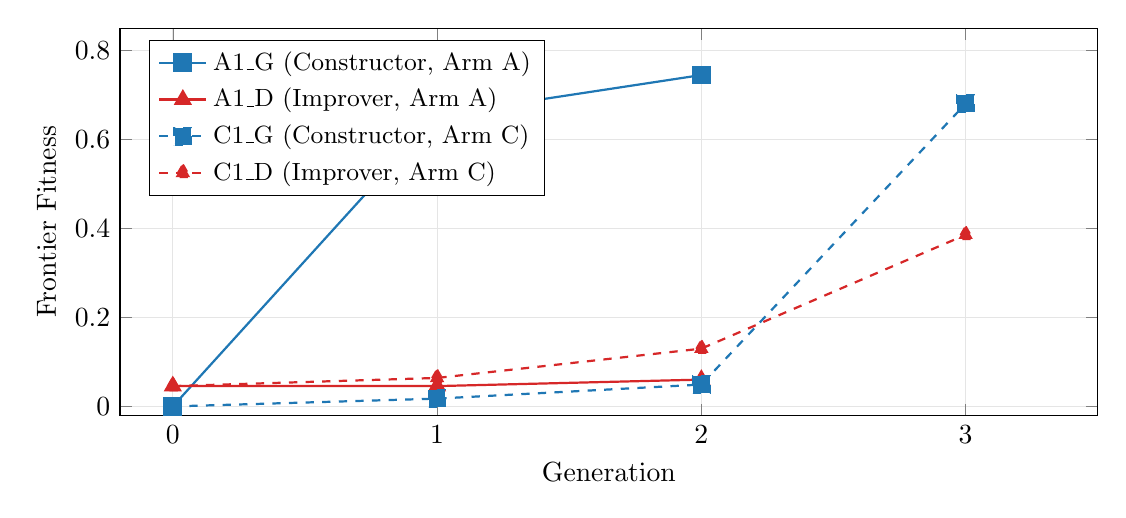
\begin{tikzpicture}
\begin{axis}[
    width=14cm, height=6.5cm,
    xlabel={Generation}, ylabel={Frontier Fitness},
    legend pos=north west,
    legend style={font=\small,cells={anchor=west},row sep=1pt},
    grid=both, grid style={gray!20},
    xmin=-0.2, xmax=3.5, ymin=-0.02, ymax=0.85,
    xtick={0,1,2,3}, every axis plot/.append style={thick,mark size=3pt},
  ]
  \addplot[color=popA,mark=square*] coordinates {(0,0.00035) (1,0.65460) (2,0.74482)};
  \addlegendentry{A1\_G (Constructor, Arm A)}
  \addplot[color=popB,mark=triangle*] coordinates {(0,0.04600) (1,0.04600) (2,0.06059)};
  \addlegendentry{A1\_D (Improver, Arm A)}
  \addplot[color=popA,mark=square*,dashed] coordinates {(0,0.00035) (1,0.01786) (2,0.04947) (3,0.68044)};
  \addlegendentry{C1\_G (Constructor, Arm C)}
  \addplot[color=popB,mark=triangle*,dashed] coordinates {(0,0.04600) (1,0.06433) (2,0.13017) (3,0.38588)};
  \addlegendentry{C1\_D (Improver, Arm C)}
\end{axis}
\end{tikzpicture}
\caption{Early arms-race (pairs A1 and C1).  Constructors (blue) jump quickly once they find good configurations.  Improvers (red) increase more gradually.  The gap = current ``arms-race advantage.''}
\label{fig:trajectory}
\end{figure}

% ═══════════════════════════════════════════════════════════
\section{Complete Information Flow}
% ═══════════════════════════════════════════════════════════

\begin{figure}[H]
\centering
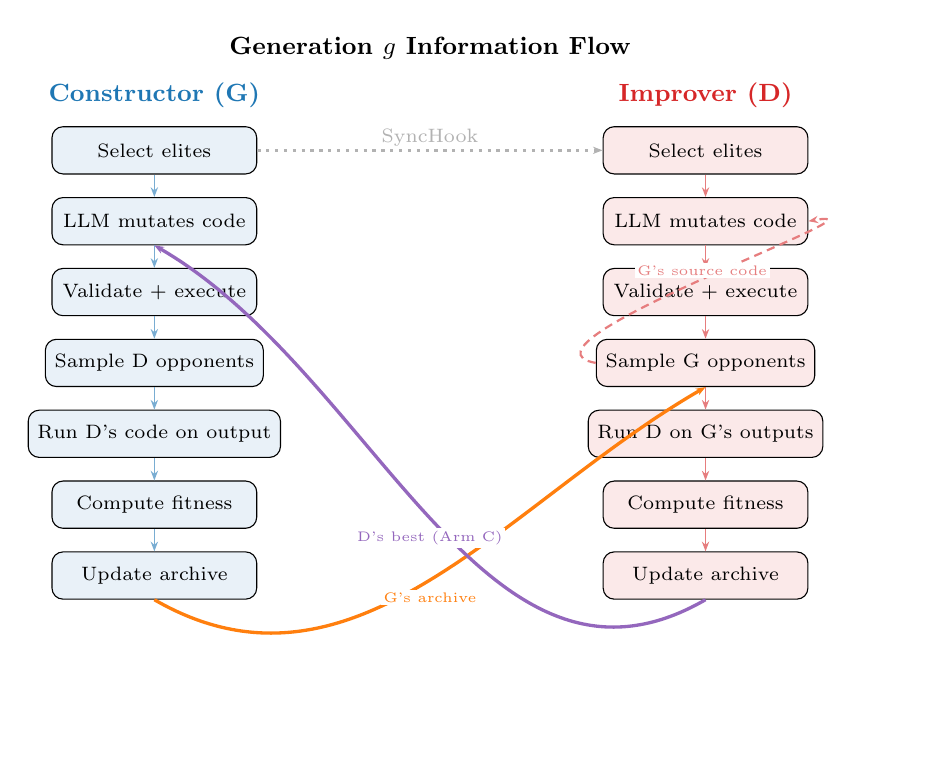
\begin{tikzpicture}[
    phase/.style={draw,rounded corners=4pt,fill=#1!10,
      minimum width=2.6cm,minimum height=0.6cm,font=\scriptsize},
    phase/.default=stageblue,
    arrow/.style={-{Stealth[length=3.5pt]},semithick},
    clbl/.style={font=\tiny,fill=white,inner sep=1pt},
    >=Stealth
  ]

  \node[font=\bfseries\small] at (0,5.8) {Generation $g$ Information Flow};

  % G column
  \node[font=\bfseries\small,popA] at (-3.5,5.2) {Constructor (G)};
  \node[phase=popA] (g1) at (-3.5,4.5) {Select elites};
  \node[phase=popA] (g2) at (-3.5,3.6) {LLM mutates code};
  \node[phase=popA] (g3) at (-3.5,2.7) {Validate + execute};
  \node[phase=popA] (g4) at (-3.5,1.8) {Sample D opponents};
  \node[phase=popA] (g5) at (-3.5,0.9) {Run D's code on output};
  \node[phase=popA] (g6) at (-3.5,0.0) {Compute fitness};
  \node[phase=popA] (g7) at (-3.5,-0.9) {Update archive};
  \foreach \a/\b in {g1/g2, g2/g3, g3/g4, g4/g5, g5/g6, g6/g7} {
    \draw[arrow,popA!60] (\a) -- (\b); }

  % D column
  \node[font=\bfseries\small,popB] at (3.5,5.2) {Improver (D)};
  \node[phase=popB] (d1) at (3.5,4.5) {Select elites};
  \node[phase=popB] (d2) at (3.5,3.6) {LLM mutates code};
  \node[phase=popB] (d3) at (3.5,2.7) {Validate + execute};
  \node[phase=popB] (d4) at (3.5,1.8) {Sample G opponents};
  \node[phase=popB] (d5) at (3.5,0.9) {Run D on G's outputs};
  \node[phase=popB] (d6) at (3.5,0.0) {Compute fitness};
  \node[phase=popB] (d7) at (3.5,-0.9) {Update archive};
  \foreach \a/\b in {d1/d2, d2/d3, d3/d4, d4/d5, d5/d6, d6/d7} {
    \draw[arrow,popB!60] (\a) -- (\b); }

  % Cross arrows (spread out to avoid overlap)
  \draw[arrow,highlight,very thick]
    (g7.south) to[out=-30,in=-150] node[clbl,below,yshift=-3pt] {G's archive} (d4.south);
  \draw[arrow,armC,very thick]
    (d7.south) to[out=-150,in=-30] node[clbl,below,yshift=-3pt] {D's best (Arm~C)} (g2.south);
  \draw[arrow,popB!60,densely dashed,thick]
    (d4.west) to[out=170,in=10] node[clbl,above] {G's source code} (d2.east);

  % Sync
  \draw[arrow,gray!60,very thick,dotted]
    (g1.east) -- node[clbl,above] {\scriptsize SyncHook} (d1.west);
\end{tikzpicture}
\caption{Full information flow per generation.  Dotted = sync barrier.  Orange = G's archive to D.  Purple = D's feedback to G.  Dashed red = source injection.}
\label{fig:infoflow}
\end{figure}

% ═══════════════════════════════════════════════════════════
\section{Pipeline Builder Construction}
% ═══════════════════════════════════════════════════════════

\begin{algorithm}[H]
\SetAlgoLined\DontPrintSemicolon
\caption{AdversarialAsymmetricPipelineBuilder}
\KwIn{role $\in$ \{constructor, improver\}, feedback\_mode $\in$ \{composition, gradient\_in\_prompt\}}
Build DefaultPipelineBuilder (standard stages)\;
Add FetchOpponentIdsStage, FetchOpponentResultsStage\;
Wire: IDs $\to$ Results $\to$ Validator; replace CallValidator with \texttt{evaluate.py}\;
\uIf{role = improver}{
  Remove: Formatter $\to$ MutationContext\;
  Add SourceCodeInjection; wire: FetchIDs $\to$ SourceCodeInjection $\to$ MutationContext\;
}
\uElseIf{role = constructor \textbf{and} mode = gradient\_in\_prompt}{
  \lIf{d\_provider is None}{\textbf{raise} ValueError}
  Remove: Formatter $\to$ MutationContext\;
  Add GradientInPrompt; wire: GradientInPrompt $\to$ MutationContext\;
}
\tcp{Arm A composition: no pipeline change --- hook at engine level}
\end{algorithm}

% ═══════════════════════════════════════════════════════════
\section{Experiment Configuration}
% ═══════════════════════════════════════════════════════════

\begin{table}[H]
\centering\small
\begin{tabular}{@{}ll@{}}
\toprule
\textbf{Parameter} & \textbf{Value} \\
\midrule
Max generations & 50 \\
Elites / mutations per gen & 8 / 8 \\
$n_{\text{opponents}}$ & 1 \\
\texttt{source\_prompt\_k} & 1 \\
Stage / DAG timeout & 3000\,s / 7200\,s \\
LLM & Qwen3-235B-A22B-Thinking \\
Mutation mode & rewrite (full program) \\
Archive re-evaluation & false \\
\midrule
Stopping rule & Gen 50 or futility at gen 25 \\
\bottomrule
\end{tabular}
\caption{Key parameters from \texttt{experiment.yaml}.}
\end{table}

% ═══════════════════════════════════════════════════════════
\section{Class Hierarchy}
% ═══════════════════════════════════════════════════════════

\begin{figure}[H]
\centering
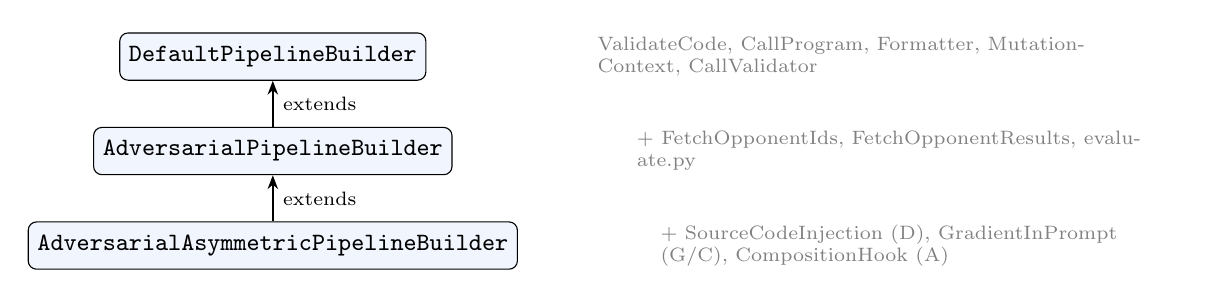
\begin{tikzpicture}[
    cls/.style={draw,rounded corners=3pt,fill=stageblue!8,
      minimum height=0.6cm,font=\small\ttfamily},
    arrow/.style={-{Stealth[length=5pt]},thick},
    ann/.style={font=\scriptsize,text=gray,text width=6.5cm,anchor=west},
    >=Stealth
  ]

  \node[cls,minimum width=3.8cm] (default) at (0,2.4) {DefaultPipelineBuilder};
  \node[cls,minimum width=4.5cm] (adv) at (0,1.2) {AdversarialPipelineBuilder};
  \node[cls,minimum width=6cm] (asym) at (0,0) {AdversarialAsymmetricPipelineBuilder};

  \draw[arrow] (asym) -- node[right,font=\scriptsize] {extends} (adv);
  \draw[arrow] (adv) -- node[right,font=\scriptsize] {extends} (default);

  \node[ann] at (4,2.4) {ValidateCode, CallProgram, Formatter, MutationContext, CallValidator};
  \node[ann] at (4.5,1.2) {+ FetchOpponentIds, FetchOpponentResults, evaluate.py};
  \node[ann] at (4.8,0) {+ SourceCodeInjection (D), GradientInPrompt (G/C), CompositionHook (A)};
\end{tikzpicture}
\caption{Pipeline builder hierarchy. Each level adds capabilities.}
\label{fig:hierarchy}
\end{figure}

% ═══════════════════════════════════════════════════════════
\section{Key Design Decisions}
% ═══════════════════════════════════════════════════════════

\begin{designbox}[title={Why fork topology instead of separate lookups?}]
\texttt{FetchOpponentIdsStage} produces one ID list feeding \emph{both} the evaluation and source injection paths. This guarantees D evaluates against the \emph{same} opponents whose code it sees.  Separate lookups could sample different opponents due to archive turnover.
\end{designbox}

\begin{designbox}[title={Why Lamarckian (Arm A) vs.\ Baldwinian (Arm C)?}]
\textbf{Arm~A} directly transplants D's solution into G's archive --- fast but G never sees D's code (black-box transfer).  \textbf{Arm~C} shows D's full source code in G's prompt --- G has white-box access and its LLM decides how to defend.  The central question: does seeing the opponent's strategy (Arm~C) or receiving its solution directly (Arm~A) produce stronger configurations?
\end{designbox}

% ═══════════════════════════════════════════════════════════
\section{Summary}
% ═══════════════════════════════════════════════════════════

\begin{table}[H]
\centering\small
\begin{tabular}{@{}p{4.5cm}p{9.5cm}@{}}
\toprule
\textbf{Component} & \textbf{Purpose} \\
\midrule
EvolutionEngine & MAP-Elites loop with pre-step hooks \\
AdversarialPipelineBuilder & Adds opponent fetching + evaluation \\
AsymmetricPipelineBuilder & Source injection (D) + gradient prompt (G/C) \\
RedisOpponentArchiveProvider & Cross-population reads with softmax sampling \\
SourceCodeInjectionStage & White-box: D sees G's Python code \\
GradientInPromptStage & White-box: G sees D's source code (Arm~C) \\
CompositionInjectionHook & Lamarckian: D's code into G's archive \\
ProgressBasedSyncHook & Sync barrier with asymmetric ratios \\
\bottomrule
\end{tabular}
\end{table}

The system achieves adversarial co-evolution through:
\textbf{(1)}~separation of concerns (Redis-only coupling);
\textbf{(2)}~bidirectional white-box access (D sees G's code; G sees D's code in Arm~C);
\textbf{(3)}~modular pipelines (new stages without touching the engine);
\textbf{(4)}~robust synchronization (progress-based, deadlock-safe).

\vfill
\begin{center}
\footnotesize
Report generated from live codebase analysis.\\
\texttt{heilbron/asymmetric-iterations} --- PR~\#204 --- \texttt{exp/heilbron/asymmetric-iterations}\\
All code references point to \texttt{gigaevo-core-internal} source files.
\end{center}

\end{document}
